%%%%%%%%%%%%%%%%%%%%%%%%%%%%%%%%%%%%%%%%%%%%%%%%%%%
%% LaTeX book template                           %%
%% Author:  Amber Jain (http://amberj.devio.us/) %%
%% License: ISC license                          %%
%%%%%%%%%%%%%%%%%%%%%%%%%%%%%%%%%%%%%%%%%%%%%%%%%%%

\documentclass[a4paper,11pt]{book}
\usepackage[T1]{fontenc}
\usepackage[utf8]{inputenc}
\usepackage{lmodern}
%%%%%%%%%%%%%%%%%%%%%%%%%%%%%%%%%%%%%%%%%%%%%%%%%%%%%%%%%
% Source: http://en.wikibooks.org/wiki/LaTeX/Hyperlinks %
%%%%%%%%%%%%%%%%%%%%%%%%%%%%%%%%%%%%%%%%%%%%%%%%%%%%%%%%%
\usepackage{hyperref}
\usepackage{graphicx}
\usepackage[english]{babel}

\usepackage{epigraph}

\usepackage{listings} 
\lstset{language=C++} 

\usepackage{courier}

\usepackage{xcolor}


%%%%%%%%%%%%%%%%%%%%%%%%%%%%%%%%%%%%%%%%%%%%%%%%%%%%%%%%%%%%%%%%%%%%%%%%%%%%%%%%
% 'dedication' environment: To add a dedication paragraph at the start of book %
% Source: http://www.tug.org/pipermail/texhax/2010-June/015184.html            %
%%%%%%%%%%%%%%%%%%%%%%%%%%%%%%%%%%%%%%%%%%%%%%%%%%%%%%%%%%%%%%%%%%%%%%%%%%%%%%%%
\newenvironment{dedication}
{
   \cleardoublepage
   \thispagestyle{empty}
   \vspace*{\stretch{1}}
   \hfill\begin{minipage}[t]{0.66\textwidth}
   \raggedright
}
{
   \end{minipage}
   \vspace*{\stretch{3}}
   \clearpage
}



%%%%%%%%%%%%%%%%%%%%%%%%%%%%%%%%%%%%%%%%%%%%%%%%
% Chapter quote at the start of chapter        %
% Source: http://tex.stackexchange.com/a/53380 %
%%%%%%%%%%%%%%%%%%%%%%%%%%%%%%%%%%%%%%%%%%%%%%%%
\makeatletter
\renewcommand{\@chapapp}{}% Not necessary...
\newenvironment{chapquote}[2][2em]
  {\setlength{\@tempdima}{#1}%
   \def\chapquote@author{#2}%
   \parshape 1 \@tempdima \dimexpr\textwidth-2\@tempdima\relax%
   \itshape}
  {\par\normalfont\hfill--\ \chapquote@author\hspace*{\@tempdima}\par\bigskip}
\makeatother

%%%%%%%%%%%%%%%%%%%%%%%%%%%%%%%%%%%%%%%%%%%%%%%%%%%
% First page of book which contains 'stuff' like: %
%  - Book title, subtitle                         %
%  - Book author name                             %
%%%%%%%%%%%%%%%%%%%%%%%%%%%%%%%%%%%%%%%%%%%%%%%%%%%

% Book's title and subtitle
\title{\Huge \textbf{Sample Book Title}  \footnote{This is a footnote.} \\ \huge Sample book subtitle \footnote{This is yet another footnote.}}
% Author
\author{\textsc{First-name Last-name}\thanks{\url{www.example.com}}}

\usepackage{blindtext}

\usepackage{caption}
\captionsetup{justification=centering}

% Bibliography
\usepackage[style=alphabetic,sorting=nyt,sortcites=true,autopunct=true,babel=hyphen,hyperref=true,abbreviate=false,backref=true,backend=biber]{biblatex}
\addbibresource{bibliography.bib} % BibTeX bibliography file
\defbibheading{bibempty}{}

\begin{document}

\frontmatter
\maketitle

%%%%%%%%%%%%%%%%%%%%%%%%%%%%%%%%%%%%%%%%%%%%%%%%%%%%%%%%%%%%%%%
% Add a dedication paragraph to dedicate your book to someone %
%%%%%%%%%%%%%%%%%%%%%%%%%%%%%%%%%%%%%%%%%%%%%%%%%%%%%%%%%%%%%%%
\begin{dedication}
Dedicated to Calvin and Hobbes.
\end{dedication}

%%%%%%%%%%%%%%%%%%%%%%%%%%%%%%%%%%%%%%%%%%%%%%%%%%%%%%%%%%%%%%%%%%%%%%%%
% Auto-generated table of contents, list of figures and list of tables %
%%%%%%%%%%%%%%%%%%%%%%%%%%%%%%%%%%%%%%%%%%%%%%%%%%%%%%%%%%%%%%%%%%%%%%%%
\tableofcontents
\listoffigures
\listoftables

\mainmatter

%%%%%%%%%%%
% Preface %
%%%%%%%%%%%
\chapter*{Kata Pengantar}

Lorem ipsum dolor sit amet, consectetur adipiscing elit. Duis risus ante, auctor et pulvinar non, posuere ac lacus. Praesent egestas nisi id metus rhoncus ac lobortis sem hendrerit. Etiam et sapien eget lectus interdum posuere sit amet ac urna.

\section*{Un-numbered sample section}
Lorem ipsum dolor sit amet, consectetur adipiscing elit. Duis risus ante, auctor et pulvinar non, posuere ac lacus. Praesent egestas nisi id metus rhoncus ac lobortis sem hendrerit. Etiam et sapien eget lectus interdum posuere sit amet ac urna. Aliquam pellentesque imperdiet erat, eget consectetur felis malesuada quis. Pellentesque sollicitudin, odio sed dapibus eleifend, magna sem luctus turpis.

\section*{Another sample section}
Lorem ipsum dolor sit amet, consectetur adipiscing elit. Duis risus ante, auctor et pulvinar non, posuere ac lacus. Praesent egestas nisi id metus rhoncus ac lobortis sem hendrerit. Etiam et sapien eget lectus interdum posuere sit amet ac urna. Aliquam pellentesque imperdiet erat, eget consectetur felis malesuada quis. Pellentesque sollicitudin, odio sed dapibus eleifend, magna sem luctus turpis, id aliquam felis dolor eu diam. Etiam ullamcorper, nunc a accumsan adipiscing, turpis odio bibendum erat, id convallis magna eros nec metus.

\section*{Structure of book}
% You might want to add short description about each chapter in this book.
Each unit will focus on <SOMETHING>.

\section*{About the companion website}
The website\footnote{\url{https://github.com/amberj/latex-book-template}} for this file contains:
\begin{itemize}
  \item A link to (freely downlodable) latest version of this document.
  \item Link to download LaTeX source for this document.
  \item Miscellaneous material (e.g. suggested readings etc).
\end{itemize}

%%%%%%%%%%%%%%%%%%%%%%%%%%%%%%%%%%%%
% Give credit where credit is due. %
% Say thanks!                      %
%%%%%%%%%%%%%%%%%%%%%%%%%%%%%%%%%%%%
\section*{Acknowledgements}
\begin{itemize}
\item A special word of thanks goes to Professor Don Knuth\footnote{\url{http://www-cs-faculty.stanford.edu/~uno/}} (for \TeX{}) and Leslie Lamport\footnote{\url{http://www.lamport.org/}} (for \LaTeX{}).
\item I'll also like to thank Gummi\footnote{\url{http://gummi.midnightcoding.org/}} developers and LaTeXila\footnote{\url{http://projects.gnome.org/latexila/}} development team for their awesome \LaTeX{} editors.
\item I'm deeply indebted my parents, colleagues and friends for their support and encouragement.
\end{itemize}
\mbox{}\\
%\mbox{}\\
\noindent Amber Jain \\
\noindent \url{http://amberj.devio.us/}

%%%%%%%%%%%%%%%%
% NEW CHAPTER! %
%%%%%%%%%%%%%%%%


%----------------------------------------------------------------------------------------
%	BAB
%----------------------------------------------------------------------------------------

\chapter{Mengenal C++ dan OpenCV}\label{dasarC++OpenCV}

\section{Pengantar}
Dari sekian banyak bahasa pemrograman yang ada, terdapat beberapa bahasa pemrograman yang populer. Dalam Gambar \ref{fig:bahasa}, ditampilkan sepuluh besar bahasa pemrograman paling populer pada tahun 2015 yang dirangkumkan dari \cite{cass_2015, ogrady_2015, tiobe_2015}. Untuk menggaris bawahi, warna kuning digunakan untuk menandai bahasa pemrograman yang masuk 5 besar dalam IEEE Spectrum, Redmonk, dan Tiobe, sedangkan warna hijau digunakan untuk menandai bahasa yang selalu masuk 5 besar dalam setiap survey.

Dari Gambar \ref{fig:bahasa}, dapat dilihat bahwa Java, C++, Python, dan C\# adalah bahasa pemrograman yang paling populer menurut ketiga survey tersebut. Dari keempat bahasa pemrograman tersebut, kebetulan semuanya mendukung pengolahan citra digital. Jadi, bahasa mana yang akan anda gunakan untuk keperluan pengolahan citra, penulis menyerahkan sepenuhnya pada pembaca. Meski demikian, dalam buku ini, penulis memilih satu bahasa pemrograman, yaitu C++. Alasan dipilihnya C++ dalam buku ini karena C++ adalah bahasa \textit{native} yang bisa digunakan dalam desktop, embedded dan mobile. Karena sifatnya yang \textit{native}, waktu eksekusinya lebih cepat dibandingkan dengan bahasa non-native seperti Java dan Python. 

Alasan lain digunakannya C++ adalah karena bahasa ini mendukung OpenCV. OpenCV yang merupakan singkatan dari Open Source Computer vision merupakan sebuah library yang banyak sekali digunakan untuk pengolahan citra digital karena performanya yang sangat bagus serta library yang sangat lengkap. OpenCV sendiri pertama kali dikembangkan oleh Intel dan direlease pertama kali pada bulan Juni tahun 2000. Pada perkembangan selanjutnya, OpenCV dikembangkan oleh Willow Garage sedangkan pada saat buku ini ditulis, OpenCV dikembangkan oleh Itseez\footnote{https://en.wikipedia.org/wiki/OpenCV}. OpenCV dapat diunduh di http://opencv.org/. Pada saat buku ini ditulis, sistem operasi yang sudah didukung oleh OpenCV adalah Windows, Linux, MacOS, Android dan iOS.

\begin{figure}
\centering
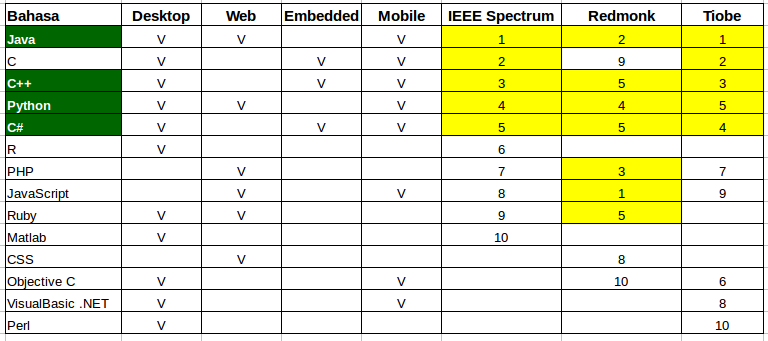
\includegraphics[width=\columnwidth]{gambar/arw_bahasa_populer}
\centering
\caption{Sepuluh Besar Bahasa Pemrograman yang Paling Populer di Dunia (2015)}
\label{fig:bahasa}
\end{figure}


Untuk IDE (\textit{Integrated Development Environment}), atau program yang digunakan untuk menulis program C++ dan OpenCV, anda bisa menggunakan IDE apapun yang anda suka (bisa notepad, notepad++, Eclipse, Netbeans, GEdit, atau apapun). Penulis sendiri cenderung lebih senang dengan \textit{the hard core way} yaitu dengan menggunakan terminal dan gedit. Meski demikian, penulis membebaskan pembaca untuk menggunakan IDE apapun yang disukai pembaca. Dengan demikian, maka di sini penulis tidak akan membahas tentang penggunaan atau interface IDE tertentu. Jika pembaca merasa kesulitan dalam penggunaan IDE yang digunakan, mohon merujuk pada sumber yang lain.

Apabila anda sudah familiar dengan C++ dan OpenCV, maka anda bisa melanjutkan ke bab selanjutnya. Jika anda sudah familiar dengan pemrograman C++ tapi belum pernah menggunakan OpenCV, penulis menyarankan untuk membaca bagian \ref{icipOpenCV} tentang struktur OpenCV. Satu hal yang perlu diingat, bahwa pemrograman adalah sebuah \textit{skill}. Cara paling baik untuk menguasai sebuah \textit{skill} adalah dengan mempraktekannya. Seseroang tidak akan bisa bersepeda jika dia hanya belajar teori bersepeda tanpa pernah menyentuh sepeda, menaiki, bahkan terjatuh dari sepeda. Sama dengan bersepeda, anda tidak akan pernah bisa belajar pemrograman kalau anda tidak pernah mempraktekkannya, berpusing ria dengan error di sana sini, dan beberapa saat kemudian tertawa sendiri ketika error tersebut sudah berhasil anda pecahkan. Beranilah untuk mencoba! Jika anda menjumpai kesalahan dalam program anda, nikmati proses \textit{debugging}nya. Ingat \textit{quotation} berikut ini:

\epigraph{FAILURE is so IMPORTANT to SUCCESS}{\textit{Jody Greene}}

\section{Mencicipi Program C++}\index{Mencicipi C++} \label{icipC++}
Seperti telah dikatakan dalam sub-bab sebelumnya, cara yang terbaik untuk belajar pemrograman adalah dengan mempraktekkannya. Dalam sub-bab ini, kita akan membuat program C++ yang sangat sederhana dan mencoba melihat lebih dalam setiap bagiannya. Pada bagian ini, penulis tidak ingin menampilkan semua aspek pemrograman C++. Untuk detail lebih lanjut tentang aspek pemrograman C++, pembaca bisa mendapatkan di sumber-sumber yang lain.

\subsection{Program 1: Halo dunia}
Berikut program pertama kita.
\lstset{
    numbers=left,
    xleftmargin=2em,
    frame=single,
    framexleftmargin=2.5em,
    basicstyle=\ttfamily\footnotesize,
    breaklines=true,
    numberstyle=\normalfont\tiny\color{gray}
    }
    


\begin{lstlisting}
// program C++ pertamaku
#include <iostream>

int main() {
    std::cout << "Halo dunia";
}
\end{lstlisting}

Selanjutnya kita akan menganalisa bagian program itu satu demi satu

\lstset{firstnumber=1}
\begin{lstlisting}
// program C++ pertamaku
\end{lstlisting}
Bagian yang diawali oleh tanda // ini disebut sebagai komentar. Apapun yang berada di belakangnya akan diabaikan oleh komputer. Meskipun bagian ini merupakan bagian yang diabaikan, komentar adalah bagian yang sangat penting bagi kita untuk memudahkan memahami alur program. Pada bagian komentar inilah, kita dapat memberikan penjelasan yang sejelas-jelasnya tentang baris-baris program yang kita buat. Tanpa adanya komentar, kita sendiri kemungkinan akan mengalami kesulitan ketika suatu saat nanti harus membuka lagi program yang sudah kita buat. Kesulitan juga akan dialami oleh orang lain ketika berusaha memahami kode program yang kita buat.

\lstset{firstnumber=2}
\begin{lstlisting}
#include <iostream>
\end{lstlisting}
Bagian selanjutnya yaitu bagian yang diawali oleh kata-kata $include$. Bagian ini merupakan bagian deklarasi yang menunjukkan library-library yang akan kita gunakan dalam kode program kita. Dalam hal ini, library yang kita masukkan adalah $iostream$.

\lstset{firstnumber=4}
\begin{lstlisting}
int main()
\end{lstlisting}
Bagian ini adalah bagian utama dari sebuah program C++. Bagian yang pertama kali dieksekusi oleh komputer adalah semua perintah yang berada di dalam fungsi main. 

\lstset{firstnumber=5}
\begin{lstlisting}
std::cout << "Halo dunia";
\end{lstlisting}
Perintah ini merupakan perintah standar C++ untuk menampilkan sesuatu ke layar. Ketika perintah ini dieksekusi, di layar akan ditampilkan kata-kata "Halo dunia" (tanpa tanda kutip).

\subsection{Program 2: Halo dunia 2}
Untuk selanjutnya, kita akan mencoba untuk sedikit lebih dalam dengan C++, yaitu dengan menempatkan perintah-perintah kita dalam sebuah fungsi. Dalam hal ini, perintah yang akan dieksekusi adalah perintah yang sama dengan latihan sebelumnya, yaitu perintah untuk menampilkan "Halo dunia". Kalau anda perhatikan, perintah untuk menampilkan "Halo dunia" tidak lagi berada di dalam main, tapi ditempatkan dalam fungsi yang kita beri nama "hello". Fungsi inilah yang kemudian dipanggil dari dalam main. Syntax lengkapnya adalah sebagai berikut:

\lstset{firstnumber=1}
\begin{lstlisting}
// program C++ keduaku
#include <iostream>

using namespace std;

void hello() {
    cout << "Halo dunia";
}

int main() {
    hello();
}

\end{lstlisting}
Karena bagian $include$ sudah dibahas sebelumnya, kita akan langsung membahas bagian program yang selanjutnya, yaitu pada fungsi hello. 

\lstset{firstnumber=4}
\begin{lstlisting}
using namespace std;
\end{lstlisting}
Bagian ini dideklarasikan agar kita tidak lagi harus menulis $std::$ dalam semua bagian dari kode kita. Jika anda perhatikan, dalam kode di program 1, kita menulis $std::cout$, tapi dalam program 2, karena kita sudah mendeklarasikan using $namespace std$, maka kita cukup menulis $cout$ saja.

\lstset{firstnumber=6}
\begin{lstlisting}
void hello() {
    cout << "Halo dunia";
}
\end{lstlisting}
Dalam C++, semua fungsi harus berada di atas main. Meskipun berada di atas main, fungsi tidak akan dieksekusi jika tidak dipanggil dalam fungsi main. Kata kunci $void$ menunjukkan bahwa fungsi ini adalah fungsi yang tidak menghasilkan sebuah nilai. Apabila kita menginginkan fungsi yang akan menghasilkan sebuah nilai, kata kunci $void$ diganti dengan tipe data dari keluaran yang diinginkan.

\lstset{firstnumber=10}
\begin{lstlisting}
int main() {
    hello();
}
\end{lstlisting}
Fungsi main memanggil fungsi hello. Ketika pemanggilan ini, maka barulah semua perintah yang berada di dalam kalang hello akan dieksekusi. Jika kalang main ini kosong, maka program tidak akan melakukan apapun meskipun di atasnya dideklarasikan fungsi hello.

\subsection{Get Your Hands Dirty}
Buatlah beberapa fungsi yang menampilkan output yang berbeda sebagai berikut:
\begin{itemize}
\item hello() --> menampilkan "Halo dunia"
\item hello2() --> menampilkan "Halo lagi"
\item hello3() --> menampilkan "Loh, kok halo lagi"
\item hello4() --> menampilkan "Udah ah"
\end{itemize}
Semua fungsi yang anda buat kemudian dipanggil dari dalam fungsi main.

\section{Mencicipi Program OpenCV}\index{Memulai OpenCV} \label{icipOpenCV}
Dalam sub-bab ini, kita akan membuat sebuah program sederhana untuk membaca dan menampilkan gambar, serta satu program sederhana lain untuk membuat negative image. 
\subsection{Program 1: Membaca dan Menampilkan Gambar}
Ambil gambar yang anda suka dari folder di komputer anda atau dari internet. Dalam contoh saya, saya menggunakan gambar buah-buahan dengan nama file fruits.png. anda bisa mendapatkan file yang dimaksud di folder gambar. Kode programnya adalah sebagai berikut.

\begin{minipage}[c]{0.95\textwidth}
\begin{lstlisting}
#include <iostream>
#include <opencv2/opencv.hpp>

using namespace cv;
using namespace std;

int main() {
    Mat buah = imread("../gambar/fruits.png");
    
    namedWindow("Gambar buah", WINDOW_AUTOSIZE);
    imshow("Gambar buah", buah);
    
    waitKey();
}
\end{lstlisting}
\end{minipage}

Bagian yang pertama akan kita bahas adalah deklarasi variabel untuk menampung gambar, yaitu

\begin{lstlisting}
Mat buah
\end{lstlisting}
Perhatikan bahwa variabel buah disimpan bukan dalam tipe data dasar (seperti int, char, dll), bukan pula dalam bentuk Array. Dalam OpenCV, tipe data yang digunakan untuk menyimpan gambar adalah tipe data Mat.

\begin{lstlisting}
imread("../gambar/fruits.png");
\end{lstlisting}
Bagian ini digunakan untuk membaca gambar dalam path yang diberikan. Dalam hal ini, path-nya adalah ../gambar/fruits.png, yang berarti bahwa gambar yang akan dibaca adalah di folder gambar yang nama file-nya adalah fruits.png. Tanda titik dua (..) menunjukkan bahwa folder gambar tersebut tidak berada di dalam folder tersebut, tapi berada di dalam folder induknya.

\begin{figure}
\centering
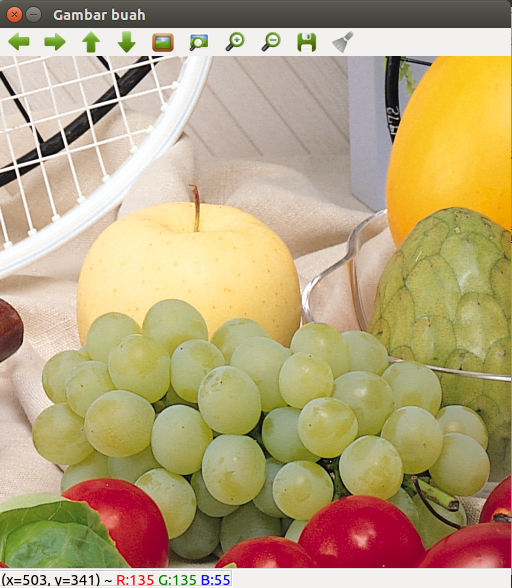
\includegraphics[width=0.5\columnwidth]{gambar/c1_fruit}
\caption{Tampilan Program 3}
\label{fig:buah}
\end{figure}

\begin{lstlisting}
namedWindow("Gambar buah", WINDOW_AUTOSIZE);
imshow("Gambar buah", buah);
\end{lstlisting}
Perintah-perintah ini digunakan untuk menampilkan gambar. Perintah namedWindow digunakan untuk membuat objek OpenCV window. Parameter pertama, yaitu "Gambar buah" digunakan untuk memberi nama window tersebut, sedangkan parameter kedua yaitu $WINDOW\_AUTORESIZE$ digunakan untuk menentukan apakah ukuran dari window tersebut bisa diubah atau tidak. Perintah selanjutnya yaitu imshow digunakan untuk menampilkan gambar yang disimpan dalam variabel buah. Judul dari jendela yang menampilkan gambar buah itu adalah "Gambar buah".

\subsection{Program 2: Membuat Negative Image}
Dalam program OpenCV yang kedua ini, kita akan membuat program untuk menghasilkan citra negatif (negative image). Untuk membuat gambar negatif, kita mengurangkan nilai intensitas masing-masing pixel dengan nilai maksimum dari intensitas yaitu 255. Sebagai contoh, jika intensitas sebuah pixel di koordinat (100, 100) adalah 200, maka pixel negatifnya adalah 255 - 200 = 55. 

Perlu dicatat bahwa gambar yang kita gunakan di sini adalah gambar RGB, dimana setiap pixelnya diwakili oleh tiga nilai, yaitu merah (Red), hijau (Green) dan biru (Blue). Kalau dalam program lain semacam matlab, susunan byte-nya dimulai dari merah, hijau, lalu biru (RGB). Akan tetapi, dalam opencv, susunan byte-nya dibalik, yaitu dimulai dari biru, hijau, kemudian merah (BGR). Kode lengkapnya adalah sebagai berikut:

\begin{lstlisting}
#include <iostream>
#include <opencv2/opencv.hpp>

using namespace cv;
using namespace std;

int main() {
    Mat buah = imread("../gambar/fruits.png");
    Mat buahInv = Mat::zeros(buah.size(), buah.type());

    for (int i=0; i<buah.rows; i++) {
        for (int j=0; j<buah.cols; j++) {
            for (int k=0; k<3; k++) {
                buahInv.at<Vec3b>(i,j)[k] = 255 - 
                    buah.at<Vec3b>(i,j)[k];
            }
        }
    }
	
    namedWindow("Gambar buah", WINDOW_AUTOSIZE);
    imshow("Gambar buah", buah);

    namedWindow("Buah Inverted", WINDOW_AUTOSIZE);
    imshow("Buah Inverted", buahInv);
    waitKey();
}
\end{lstlisting}
Kita tidak akan membahas baris demi baris. Perintah-perintah yang sudah dibahas dalam program sebelumnya tidak akan dibahas lagi. 

\begin{figure}
\centering
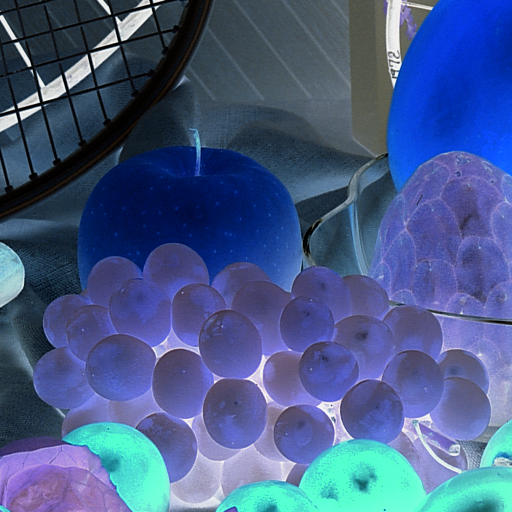
\includegraphics[width=0.5\columnwidth]{gambar/c1_buah_inverted}
\caption{Gambar Buah (citra negatif)}
\label{fig:buah_negatif}
\end{figure}

\begin{lstlisting}
Mat buahInv = Mat::zeros(buah.size(), buah.type());
\end{lstlisting}
Dalam baris perintah ini, kita membuat sebuah matrix yang berukuran sama dengan matrix buah. Matrix ini adalah matrix kosong yang isinya adalah nilai nol (zeros). Matrix ini akan kita gunakan untuk menampung nilai-nilai pixel dari gambar negatif.

\begin{lstlisting}
for (int i=0; i<buah.rows; i++) {
    for (int j=0; j<buah.cols; j++) {
        for (int k=0; k<3; k++) {
            buahInv.at<Vec3b>(i,j)[k] = 255 - 
                buah.at<Vec3b>(i,j)[k];
        }
    }
}
\end{lstlisting}
Dalam baris-baris perintah ini, kita mengakses setiap nilai pixel yang ada dalam variabel buah. Jika anda perhatikan, kita menggunakan tiga variabel yaitu i, j, dan k. Variabel i digunakan untuk mengakses baris (rows), variabel j digunakan untuk mengakses kolom (cols), sedangkan variabel k digunakan untuk mengakses kanal warna RGB (atau BGR dalam OpenCV). 

%----------------------------------------------------------------------------------------
%	BAB
%----------------------------------------------------------------------------------------

\chapter{Dasar-dasar Matrix} \label{matrix}

\section{Pengantar}
Dalam pengolahan citra, pemahaman tentang matrix dan operasinya mutlak diperlukan. Oleh karena itu, penulis merasa perlu untuk menuliskan satu bab tersendiri tentang matrix. Bab ini tidak dirancang untuk menampilkan semua teori matrix, akan tetapi hanya menampilkan bagian-bagian yang paling sering dibutuhkan dalam pengolahan citra. Teori lebih lengkap tentang matrix dapat dibaca dari sumber-sumber yang lain. 

Apabila anda sudah familiar dengan matrix dan operasinya, maka anda bisa skip bab ini dan melanjutkan ke bab selanjutnya. Apabila anda belum pernah sama sekali atau ingin mengulangi pelajaran tentang matrix, penulis sangat menganjurkan untuk membaca dan memahami bab ini terlebih dahulu.

\blindtext

\section{Operasi Dasar}
\blindtext

\subsection{Penambahan dan Pengurangan}
\blindtext

\subsection{Perkalian}
\blindtext

\subsection{Transformasi Matrix}
\blindtext

\subsection{Matrix Konvolusi}
\blindtext

%----------------------------------------------------------------------------------------
%	BAB
%----------------------------------------------------------------------------------------

\chapter{Dasar-dasar Pengolahan Citra} \label{dasarCitra}

\section{Pengantar}
\blindtext

\section{Mengenal Spektrum Elektromagnet}
\blindtext

\section{Mengenal Alat Akuisisi Citra}
\blindtext

\section{Representasi Citra}
\blindtext
\subsection{Tipe Citra Digital}
\blindtext
\subsection{Tipe Data untuk Representasi Citra}
\blindtext

\section{Color Space}
\blindtext
\subsection{RGB} % CIE, RGB, YUV, HSL/HSV, and CMYK.
\blindtext
\subsection{CMYK}
\blindtext
\subsection{HSL/HSV}
\blindtext
\subsection{CIE}
\blindtext
\subsection{YUV}
\blindtext

\section{Contrast and Brightness}
\blindtext
\subsection{Definisi Image Contrast}
\blindtext
\subsection{Contoh Implementasi Image Contrast}
\blindtext


%----------------------------------------------------------------------------------------
%	BAB
%----------------------------------------------------------------------------------------

\chapter{Noise} \label{noise}

\section{Pengantar}
\blindtext

\section{Photoelectronic Noise}
\blindtext
\subsection{Photon Noise}
\blindtext
\subsection{Thermal Noise}
\blindtext

\section{Impulse Noise}
\subsection{Salt Noise}
\blindtext
\subsection{Pepper Noise}
\blindtext
\subsection{Salt and Pepper Noise}
\blindtext
\subsection{Line Drop Noise}
\blindtext

\section{Structure Noise}
\blindtext
\subsection{Periodic, Stationary}
\blindtext
\subsection{Periodic, Nonstationary}
\blindtext
\subsection{Aperiodic}
\blindtext
\subsection{Detector Striping}
\blindtext
\subsection{Detector Banding}
\blindtext


%----------------------------------------------------------------------------------------
%	BAB
%----------------------------------------------------------------------------------------

\chapter{Mengenal Filter}

\section{Linear Filter}
\blindtext
\subsection{Blur, Sharpen}
\blindtext
\subsection{Gaussian Filter}
\blindtext
\subsection{Gradient Filter}
\blindtext
\subsection{Laplacian Filter}

\section{Non Linear Filter}
\blindtext
\subsection{Median Filter}
\blindtext
\subsection{Geometric Mean Filter}
\blindtext

\section{Non Local Filter}
\blindtext
\subsection{Image Deconvolve}
\blindtext
\subsection{Total Variation Filter}
\blindtext

\section{Frequency Based Filter}
\blindtext
\subsection{Lowpass Filter}
\blindtext
\subsection{Highpass Filter}
\blindtext

%----------------------------------------------------------------------------------------
%	BAB
%----------------------------------------------------------------------------------------

\chapter{Operasi Biner pada Gambar Digital}
\blindtext

%----------------------------------------------------------------------------------------
%	BAB
%----------------------------------------------------------------------------------------

\chapter{Deteksi Objek}
\blindtext

%----------------------------------------------------------------------------------------
%	BAB
%----------------------------------------------------------------------------------------

\chapter{Klasifikasi dan Pengenalan Pola}
\blindtext

%----------------------------------------------------------------------------------------
%	BAB
%----------------------------------------------------------------------------------------

\chapter{Klasterisasi}
\blindtext

%----------------------------------------------------------------------------------------
%	BAB
%----------------------------------------------------------------------------------------

\chapter{Image Beautification}
\blindtext

%----------------------------------------------------------------------------------------
%	BAB
%----------------------------------------------------------------------------------------

\chapter{3D Acquisition}
\blindtext

%----------------------------------------------------------------------------------------
%	BAB
%----------------------------------------------------------------------------------------

\chapter{3D Object Recognition}
\blindtext

\end{document}
